\documentclass{article}
\usepackage{graphics}

\begin{document}
\section{Commande \texttt{\char92 includegraphics}}
\label{include}
%\label{zobi}
\begin{center}
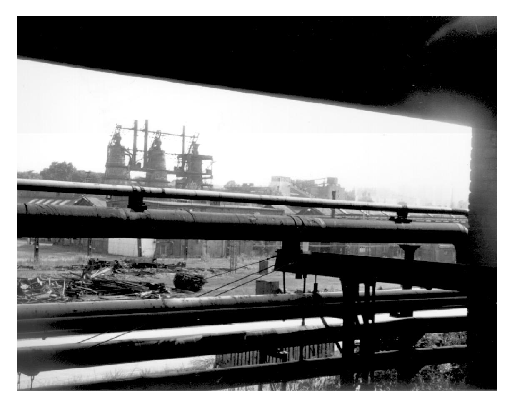
\includegraphics{HF.ps}
\end{center}

\includegraphics*[1cm,1cm]{HF.ps}
\label{autre}

\section{Commandes \texttt{\char92 scalebox} et \texttt{\char92 resizebox}}

\begin{center}
\scalebox{.5}{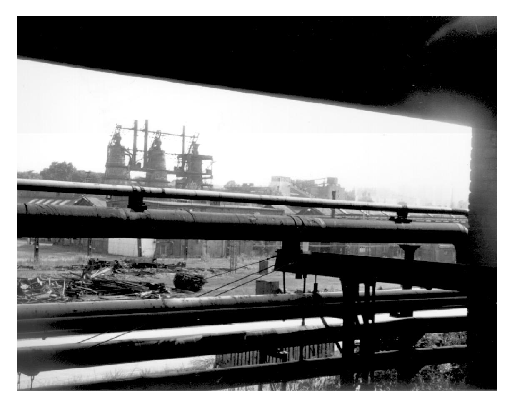
\includegraphics{HF.ps}}
\end{center}

Scaled .2 \scalebox{.2}[1]{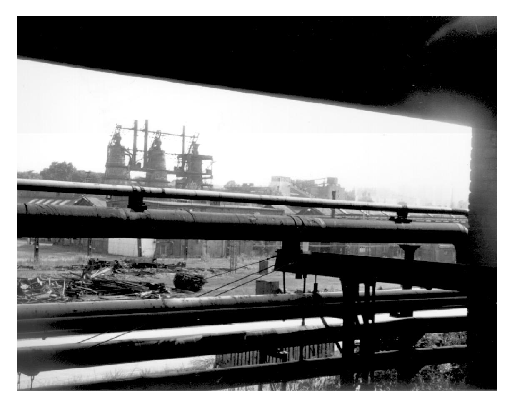
\includegraphics{HF.ps}}
Scaled .4 \scalebox{.4}[1]{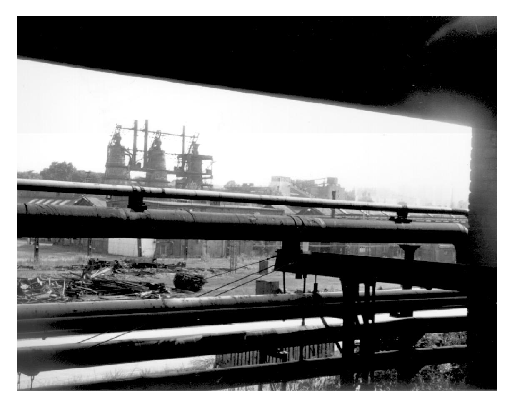
\includegraphics{HF.ps}}
Scaled .6 \scalebox{.6}[1]{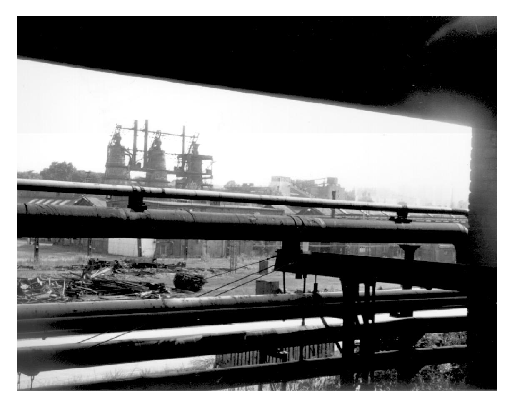
\includegraphics{HF.ps}}

\resizebox{1cm}{!}{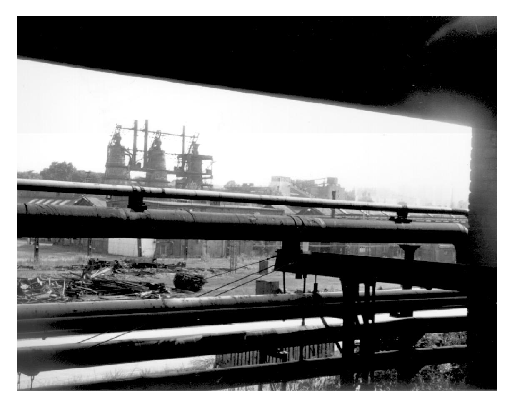
\includegraphics{HF.ps}}
\resizebox{2cm}{!}{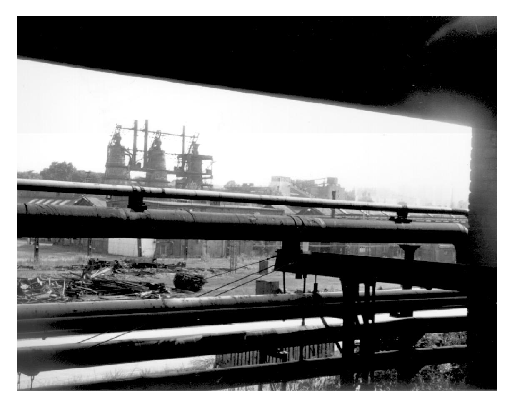
\includegraphics{HF.ps}}
\resizebox{4cm}{!}{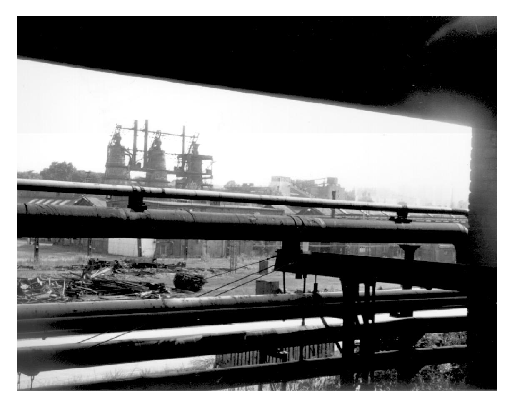
\includegraphics{HF.ps}}
\resizebox{8cm}{!}{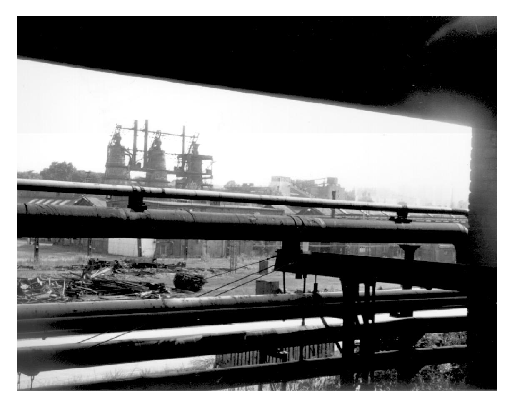
\includegraphics{HF.ps}}

\section{Transformations}
\rotatebox{45}{\scalebox{.5}{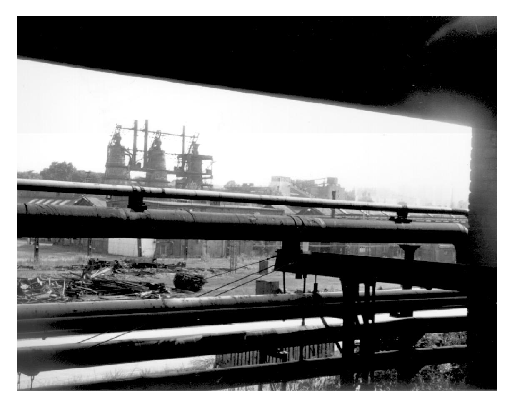
\includegraphics{HF.ps}}}
\newcommand{\monrot}[2]{\rotatebox{#1}{#2}}
\monrot{135}{\scalebox{.5}{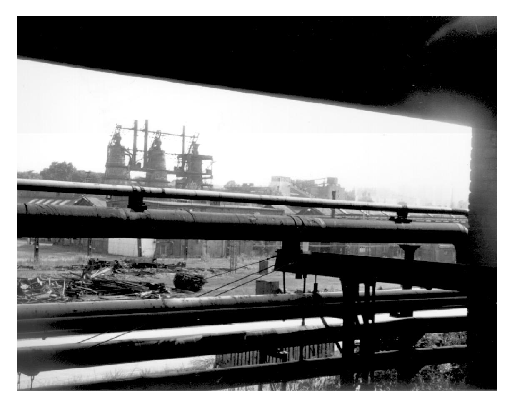
\includegraphics{HF.ps}}}



\reflectbox{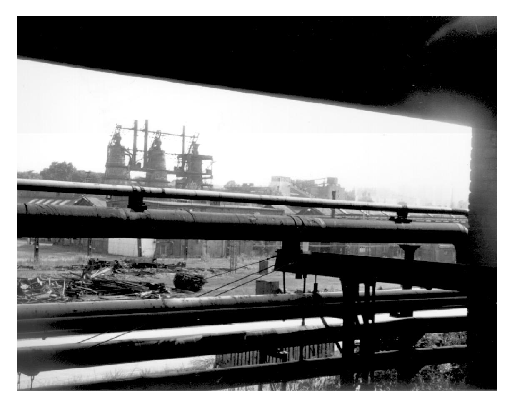
\includegraphics{HF.ps}}

La premi\`re section est~\ref{include} ou~\ref{autre}.

\end{document}
